\chapter {Marco Teórico}
\spacing{1.5}
\section {Extracción y descripción de características}
Las características de los objetos son cualidades que sirven para identificarlos  dentro de una imagen. Para poder distinguir objetos que estén en una imagen nos basamos en las características encontradas por algún algoritmo, mismas que serán encapsuladas en un descriptor. Un descriptor de un objeto es la representación, de una manera reducida, de todas las características que se pueden obtener del objeto. Esto facilitará la identificación de los diferentes objetos que existan en una imagen.\\
Para extraer las características existen diferentes métodos. Dependerá de que algoritmo se utilice pues cada uno de ellos se enfoca en encontrar diferentes características como esquinas, bordes, crestas y regiones que son más obscuras o más claras. No todos los reconocedores encontrarán las mismas características o todos los tipos de características. Para que estas características sean robustas deben poder ser encontradas aunque los objetos se encuentren rotados, escalados, con cambios de iluminación o si están parcialmente ocluidos.\\
A continuación se explicara cómo se obtienen estas características, a las cuales les llamaremos puntos característicos, por medio del algoritmo de SIFT.
\subsection{Características invariantes a transformaciones afines}
El algoritmo Scale-Invariant Feature Transform (SIFT), propuesto por Lowe en \cite{Lowe2004},  provee un método robusto para la extracción de puntos característicos que se utilizan para generar el descriptor. Los puntos que se encuentran son invariantes a diferentes transformaciones como traslación, escalamiento y rotación. Han mostrado tener un amplio rango de tolerancia a transformaciones afines, adición de ruido y cambios de iluminación. A continuación se describirán los pasos del algoritmo para la generación del conjunto de puntos característicos:
\subsubsection{Detección de puntos extremos en el Espacio-Escala} 
Se realiza una búsqueda en las imágenes en todo el espacio escala. Para localizar puntos extremos se debe identificar su ubicación y escala para volver a encontrarlos no importando la vista o tamaño del mismo objeto.\\
El espacio escala es un conjunto de imágenes, que se forman a partir de suavizar la imagen original a diferentes niveles de detalles, los cuales son definidos por un parámetro $\sigma$. Está representado por la función $L(x,y;\sigma)$ la cual se forma por la convolución de $G(x,y;\sigma)$ con la imagen original $I(x,y)$:
$$L(x,y;\sigma) = G(x,y;\sigma) * I(x,y)$$
Donde $*$ es el operador convolución en $(x,y)$, y
$$ G(x,y;\sigma) = \frac{1}{2\pi\sigma^2}e^{\frac{-(x^2+y^2)}{2\sigma^2}}$$
Para la detección de puntos extremos estables se aplica el espacio escala usando diferencias de gaussiana convolucionadas con una imagen en lugar de solo un filtro gaussiano $D(x,y;\sigma)$  que podremos calcular por la diferencia de dos escalas cercanas separadas por un factor $k$ multiplicativo:
$$D(x,y;\sigma) = \big(G(x,y;k\sigma) - G(x,y;\sigma)\big) * I(x,y)$$ $$= L(x,y;k\sigma) - L(x,y;\sigma)$$
La diferencia de gaussiana es una aproximación muy cercana a el laplaciano de gaussiana (LoG) normalizado en escala, $\sigma^2 \nabla^2 G$. La normalización hecha con el factor $\sigma^2$ es necesaria para poder asegurar que el algoritmo será invariante a los cambios en tamaño. La relación entre D y $\sigma^2 \nabla^2 G$ es una ecuación en derivadas parciales:
$$\frac{\partial G}{\partial \sigma} = \sigma \nabla^2 G$$
Podemos ver que $\nabla^2 G$ se puede calcular con una aproximación de diferencias finitas de  $\frac{\partial G}{\partial \sigma}$ usando diferencias de escalas próximas de $k\sigma$ y $\sigma$:
$$ \sigma \nabla^2 G = \frac{ \partial G}{\partial \sigma} \approx  \frac{G(x , y , k \sigma) - G( x , y, k \sigma)}{k \sigma - \sigma}$$
Y, por lo tanto:
$$ G(x , y , k \sigma) - G( x , y, k \sigma) \approx (k - 1)\sigma^2 \nabla^2 G $$
En la figura 2-1 se puede ver la construcción de $D(x,y,\sigma)$. La imagen inicial se convoluciona con diferentes mascaras gaussiana para producir imágenes separadas por un factor constante $k$ en el espacio escala. Se divide cada octava del espacio escala entre un numero entero $s$ de intervalos, quedando entonces $k= 2^\frac{1}{s}$. Se producen $s+3$  imágenes emborronadas en la pila por octava.\\
\begin{figure}[H]
	\centering
	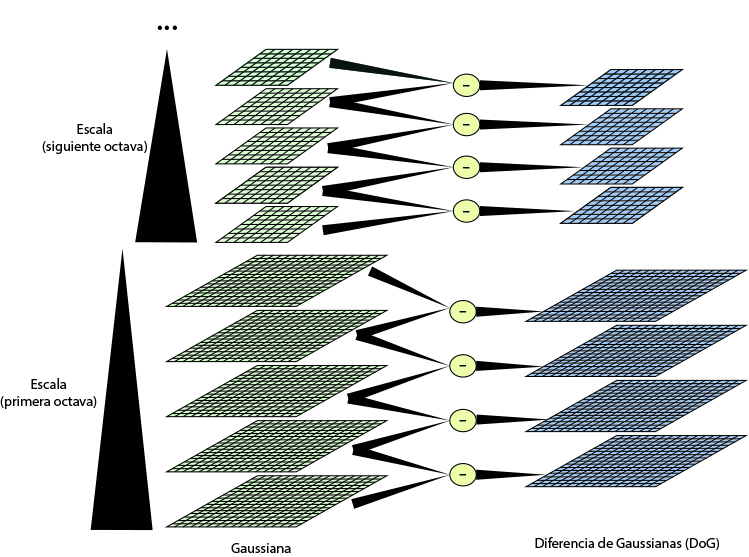
\includegraphics[height=8cm]{img/spaceScale.jpg}
	\caption{Espacio Escala de Diferencia de Gaussiana}
\end{figure}	
Para extraer las ubicaciones máximas y mínimas (puntos extremos) en $D(x,y,\sigma)$ cada punto es comparado con sus ocho vecinos en la misma imagen y con sus otros dieciocho vecinos de escala, nueve en la imagen de arriba y nueve en la imagen de abajo (Figura 2-2). Solo se selecciona el punto si es el más grande o el más pequeño de entre todos sus vecinos.
\begin{figure}[H]
	\centering
		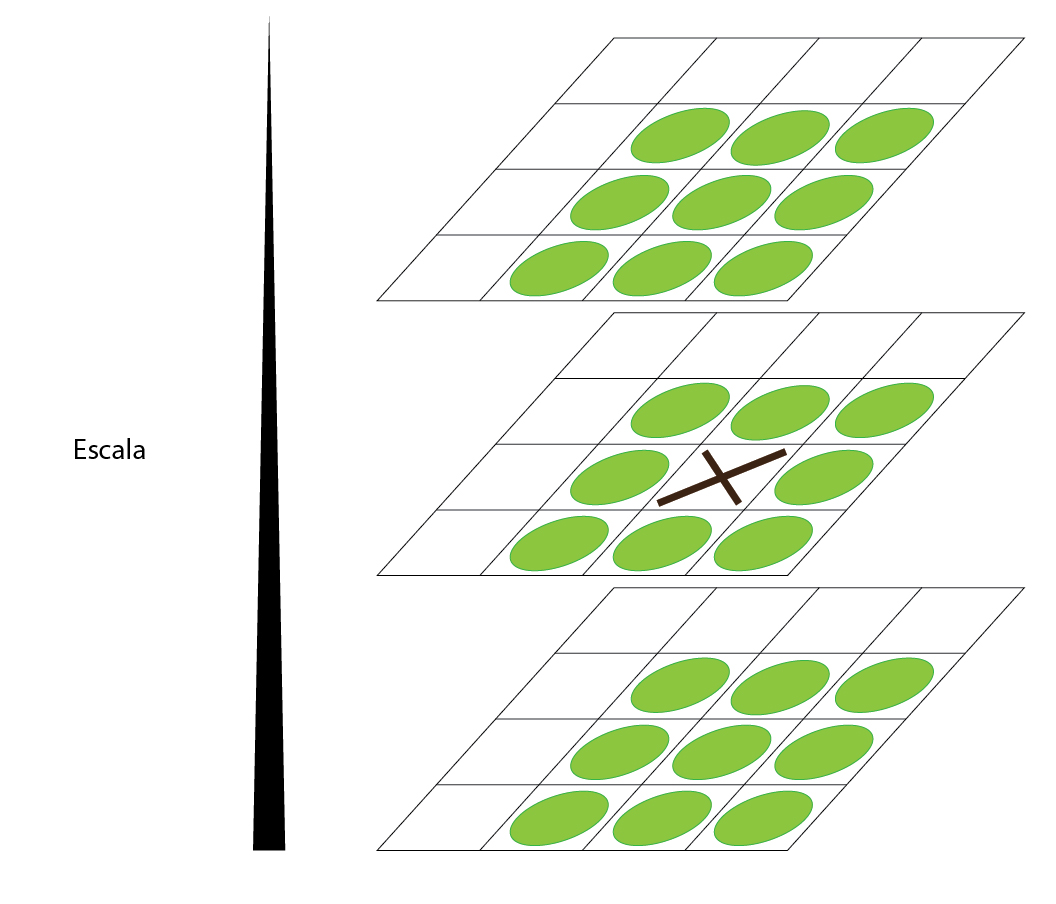
\includegraphics[height=7cm]{img/EscalaPuntosExtremos.jpg}
	\caption{Espacio Escala de Diferencia de Gaussiana}
\end{figure}
\subsubsection{Localización de puntos característicos}
Una vez que se seleccionaron los puntos extremos se aplica una medida de estabilidad sobre todos para descartar aquellos que no sean adecuados, para obtener puntos  característicos de forma precisa. Existen dos casos donde los puntos extremos anteriormente seleccionados tienen que ser eliminados:
\begin{enumerate}
	\item El punto tiene un contraste muy bajo.
	\item El punto está localizado sobre un borde.
\end{enumerate}			
Para eliminar los puntos del caso uno primero se debe obtener la serie de Taylor del espacio escala $D(x,y,\sigma)$:
$$D(X)=D +\frac{\partial D}{\partial X}^T X+ \frac{1}{2} X^T\frac{\partial^2 D}{\partial X^2} X $$
Donde la $D$ y su derivada son evaluadas en el punto $X = (x,y,\sigma)^T$. Cuando se deriva esta función respecto a $X$ y se iguala a cero podemos encontrar los valores extremos: 
$$ \hat{X} = - \frac{\partial^2 D}{\partial X^2}^{-1}\frac{\partial D}{\partial X}$$
La función que evaluará al punto extremo será, $D(\hat{X})$, la cual rechazará al punto si es de muy bajo contraste, la cual se obtiene de sustituir $\hat{X}$ en $D(X)$:
$$D(\hat{X})=D + \frac{1}{2} \frac{\partial D}{\partial X}^T \hat{X} $$ 	 
En el trabajo de Lowe \cite{Lowe2004}, se encontró experimentalmente que cualquier valor extremo menor de 0.03 puede ser descartado:
$$ |D(\hat{X})|< 0.03$$ 	 
Para el segundo caso, se utiliza una matriz Hessiana $H$ de $2\times2$ la cual se calcula en la escala y lugar del punto extremo:
$$ 
H
=
\begin{bmatrix}
	D_{xx} & D_{xy}\\
	D_{xy} & D_{yy}
\end{bmatrix}		 	
$$	
Los valores propios de H son proporcionales a las curvaturas de D. Si se toma prestado el criterio que se usa para la detección de esquinas usando el algoritmo de Harris \cite{Harris1988}, se puede evitar el cálculo de los valores propios ya que solo nos interesa su relación. Sea $\alpha$ el valor propio de mayor magnitud y $\beta$ el de menor. Entonces podemos calcular la suma de los valores propios de la diagonal de $H$ y su producto por medio del determinante:
$$Tr(H) = D_{xx} + D_{yy} = \alpha+\beta,$$ $$Det(H) = D_{xx}D_{yy}-(D_{xy})^2= \alpha\beta$$
Sea $r$ la razón de la magnitud que existe entre $\alpha$ y $\beta$, $\alpha = r\beta$. Entonces:
$$\frac{Tr(H)^2}{Det(H)}= \frac{(\alpha+\beta)^2}{\alpha\beta}= \frac{(r\beta+\beta)^2}{r\beta^2}= \frac{(r+1)^2}{r}$$
El cual solo depende de la razón de los valores propios y no de los valores individuales. El valor de $\frac{(r+1)^2}{r}$, es más pequeño cuando los valores propios son iguales e incrementa con $r$. Entonces para corroborar que la razón de las curvas principales es menor que cierto umbral $r$ sólo se necesita:
$$\frac{Tr(H)^2}{Det(H)} < \frac{(r+1)^2}{r}$$
En la publicación de Lowe \cite{Lowe2004} se encontró un valor experimental para $r=10$ que elimina los puntos extremos que tengan la razón entre las dos curvas mayor que 10.
\subsubsection{Asignación de orientación}
Por medio de la asignación de una orientación a cada punto característico, basado en propiedades locales de la imagen, el descriptor que encontremos será invariante a la rotación. La ubicación en el espacio escala del punto característico, es usada para seleccionar la imagen suavizada por una máscara gaussiana, $L$, esto provocara que sea invariante a la escala. Para cada muestra de la imagen $L(x,y)$ la magnitud del gradiente $m(x,y)$ y la orientación $\theta(x,y)$ son precalculadas por medio de diferencias de gaussiana:
$$m(x,y) = \sqrt{ \big(L(x+1,y)-L(x-1,y)\big)^2 + \big(L(x,y+1)-L(x,y-1)\big)^2 }$$		
$$\theta(x,y) =  \tan^{-1} \left(\frac{L(x,y+1)-L(x,y-1)}{L(x+1,y)-L(x-1,y)}\right)$$
Se formará un histograma de orientaciones que tendrá la orientación de los gradientes calculados en una región alrededor del punto característico. El tamaño de esta muestra dependerá de la ubicación en el espacio escala en la que se encuentre el punto característico. El histograma de orientaciones tendrá 36 divisiones cubriendo los 360 grados.\\
Cada muestra agregada se pondera por la magnitud de su gradiente y por una máscara circular gaussiana ponderada con $1.5\times\sigma$, donde la  $\sigma$ dependerá del espacio escala donde reside el punto característico.\\	
Los picos en el histograma de orientación corresponden a las direcciones dominantes de los gradientes locales. Se encuentra el pico más grande y cualquier otro pico que se encuentre en el rango de $100\% - 80\%$ del pico más grande se utiliza para hacer que el punto característico tenga una orientación (figura 2-3). Para ubicaciones con varios picos de magnitudes similares se generaran puntos característicos con la misma ubicación y escala pero con diferentes orientaciones. Solo el $15\%$ de los puntos se les asignan múltiples orientaciones, pero aun así esto contribuye mucho al momento de emparejar. Finalmente se obtiene una parábola usando como puntos tres picos cercanos entre sí, para interpolar la posición del pico con más precisión.
\begin{figure}[H]
	\centering
		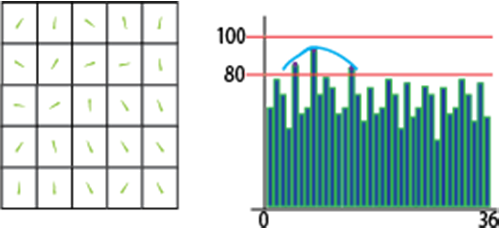
\includegraphics[height=4cm]{img/HistoOrientacion.png}
	\caption{Histograma de Orientación}
\end{figure}
\subsubsection{Descriptor de puntos característicos}
Hasta este momento se tiene una colección de puntos característicos, los cuales están formados por una ubicación, una escala y una orientación. Ahora debemos formar un descriptor que sea lo suficientemente distintivo. Para esto tenemos que tomar una muestra de la imagen al rededor del punto característico de $16\times16$ pixeles que se dividirá en una región de $4 \times 4$. Se generará un histograma de orientación de los gradientes de cada región a diferencia del histograma de orientación explicado anteriormente, el histograma sólo tiene 8 divisiones con las cuales se cubrirán los 360 grados. Igualmente se usará una ponderación gaussiana para la asignación de la magnitud al histograma (figura 2-4).\\
\begin{figure}[H]
	\centering
		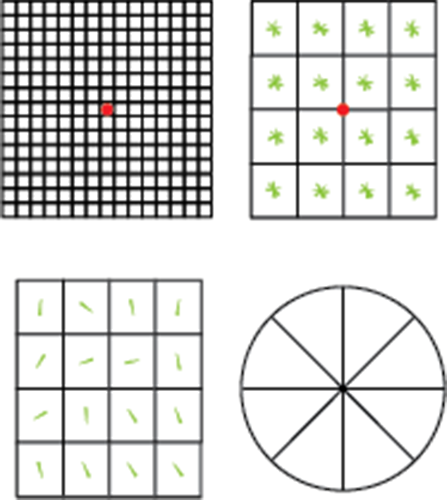
\includegraphics[height=8cm]{img/Descriptor.png}
	\caption{Descriptor}
\end{figure}
Al final, el descriptor de cada punto característico estará formado por un vector que tiene las ocho orientaciones de los $4\times4$ histogramas. Por lo tanto el tamaño del vector será de $4\times4\times8 = 128$ elementos.\\
\section {Cómputo en GPU}
Hasta hace 12 años la velocidad a la que crecía cada generación de procesadores mononúcleo era increíble, los programas eran tan rápidos como cada nueva generación de procesadores. Este crecimiento entre cada generación se detuvo. El problema es que el consumo de energía y la disipación de calor no permiten aumentar la frecuencia de reloj del procesador y el nivel de actividades por ciclo, en una sola unidad de procesamiento (CPU). Todos los productores de procesadores migraron a un nuevo modelo, los procesadores multinúcleo incrementaron el poder de procesamiento.\\
Este cambio en los procesadores tuvo un gran impacto a los programadores, la mayoría de las aplicaciones son escritas de forma secuencial porque la ejecución será paso a paso como esta descrito en el código, esto permitirá que al momento de corregir errores de programación o entender cómo funciona el programa sea más sencillo. \\
Pero un programa secuencial ejecutándose en un solo núcleo del procesador no será más rápido. Entonces los programadores ya no pueden agregar cualidades y capacidades a sus programas de forma tradicional.\\
Llega el momento de cambiar. Si se desea que la calidad de los programas siga escalando con cada generación de procesadores se deben crear programas que trabajen con múltiples hilos, cooperando todos para completar un trabajo más rápido.\\
Existen dos corrientes principales en cuanto a los procesadores multinúcleo: el primero es donde se pretende mantener la velocidad de los programas secuenciales mientras se mueven entre múltiples núcleos. La segunda se centra más en la ejecución de aplicaciones que fueron específicamente diseñadas para aprovechar todos los núcleos en el procesador al mismo tiempo, los procesadores de esta corriente tienen un gran número de núcleos pequeños que va creciendo con cada generación. Es esta rama en la que entran las unidades de procesamiento gráfico o por sus siglas en ingles GPU \cite{Kirk2010}. En la figura 2-5 podemos ver una comparación de estas dos corrientes considerando a la cantidad de operaciones de punto flotante que pueden realizar en un segundo (flops).\\
En el capítulo 3 hablaremos más a detalle sobre el cómputo en GPU especialmente de los GP-GPU de NVIDIA.\\
\begin{figure}[H]
			\centering
				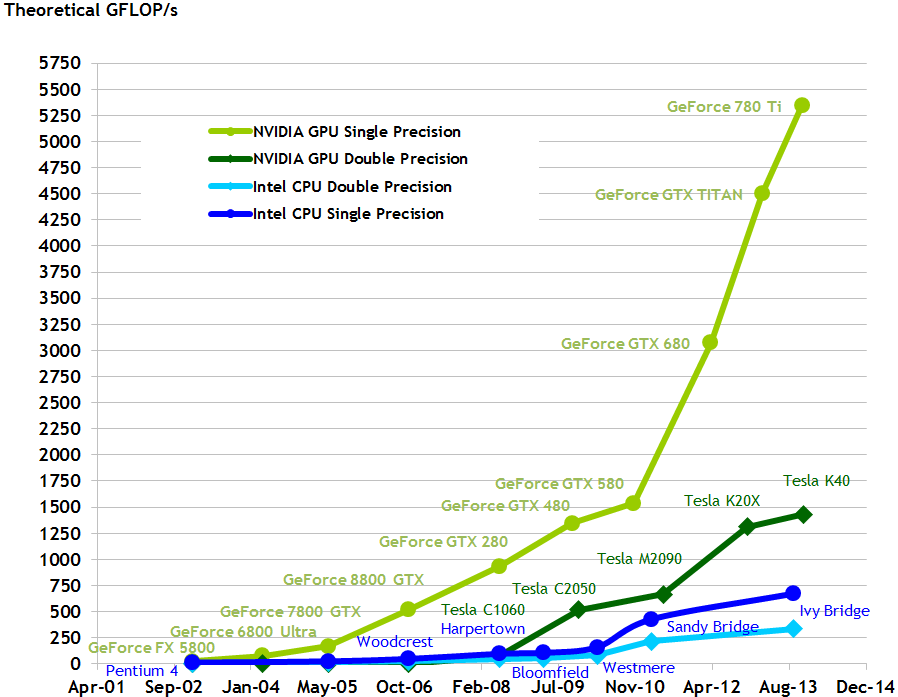
\includegraphics[height=13cm]{img/flops.png}
			\caption{Operaciones en Punto Flotante por segundo de GPU y CPU \cite{Flops}}
\end{figure}
